\subsection{Sekvensdiagrammer der anvendes i applikationsmodel for PSoC 5}
\begin{figure}[H]
	\caption{Sekvensdiagram for funktionen Gå til position}
	\label{SD:PSoC:GaaTilPos}
	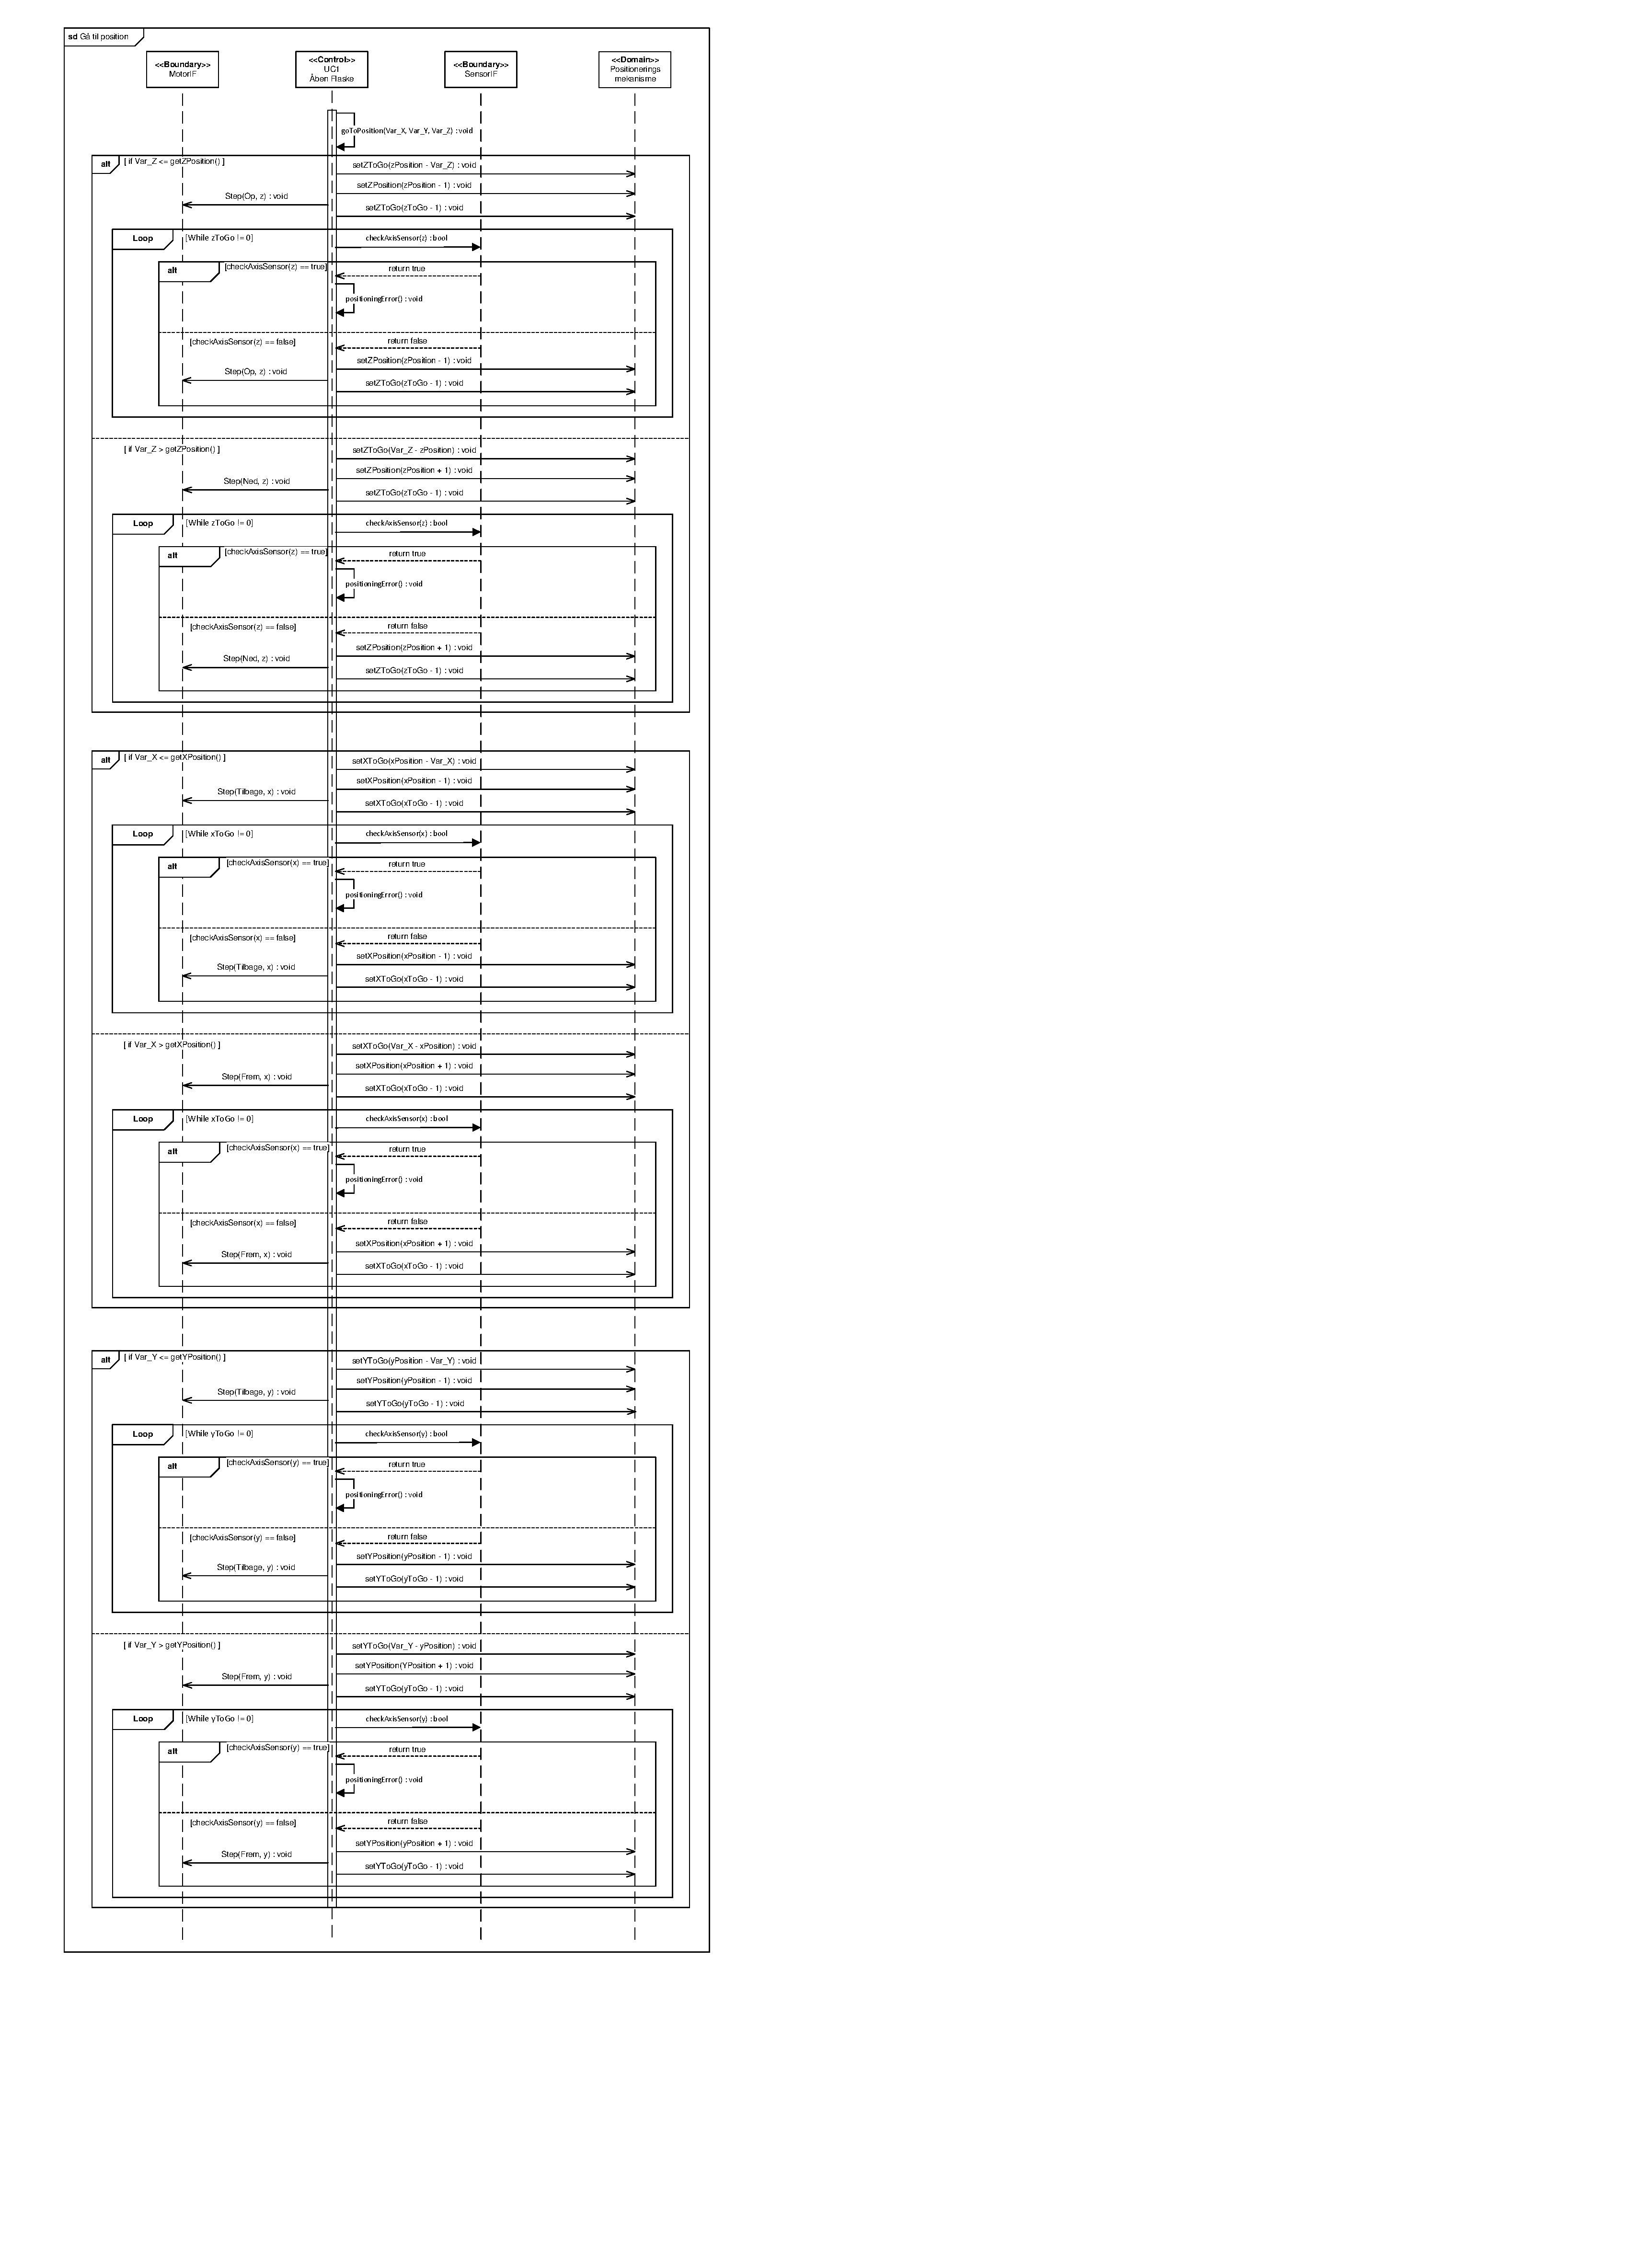
\includegraphics[scale=0.29,trim=0 0 1000 0]{APPSoC/SD-Gaa-til-position-v1}
\end{figure}

\begin{figure}[H]
	\caption{Sekvensdiagram for funktionen Scan x-aksen}
	\label{SD:PSoC:ScanX}
	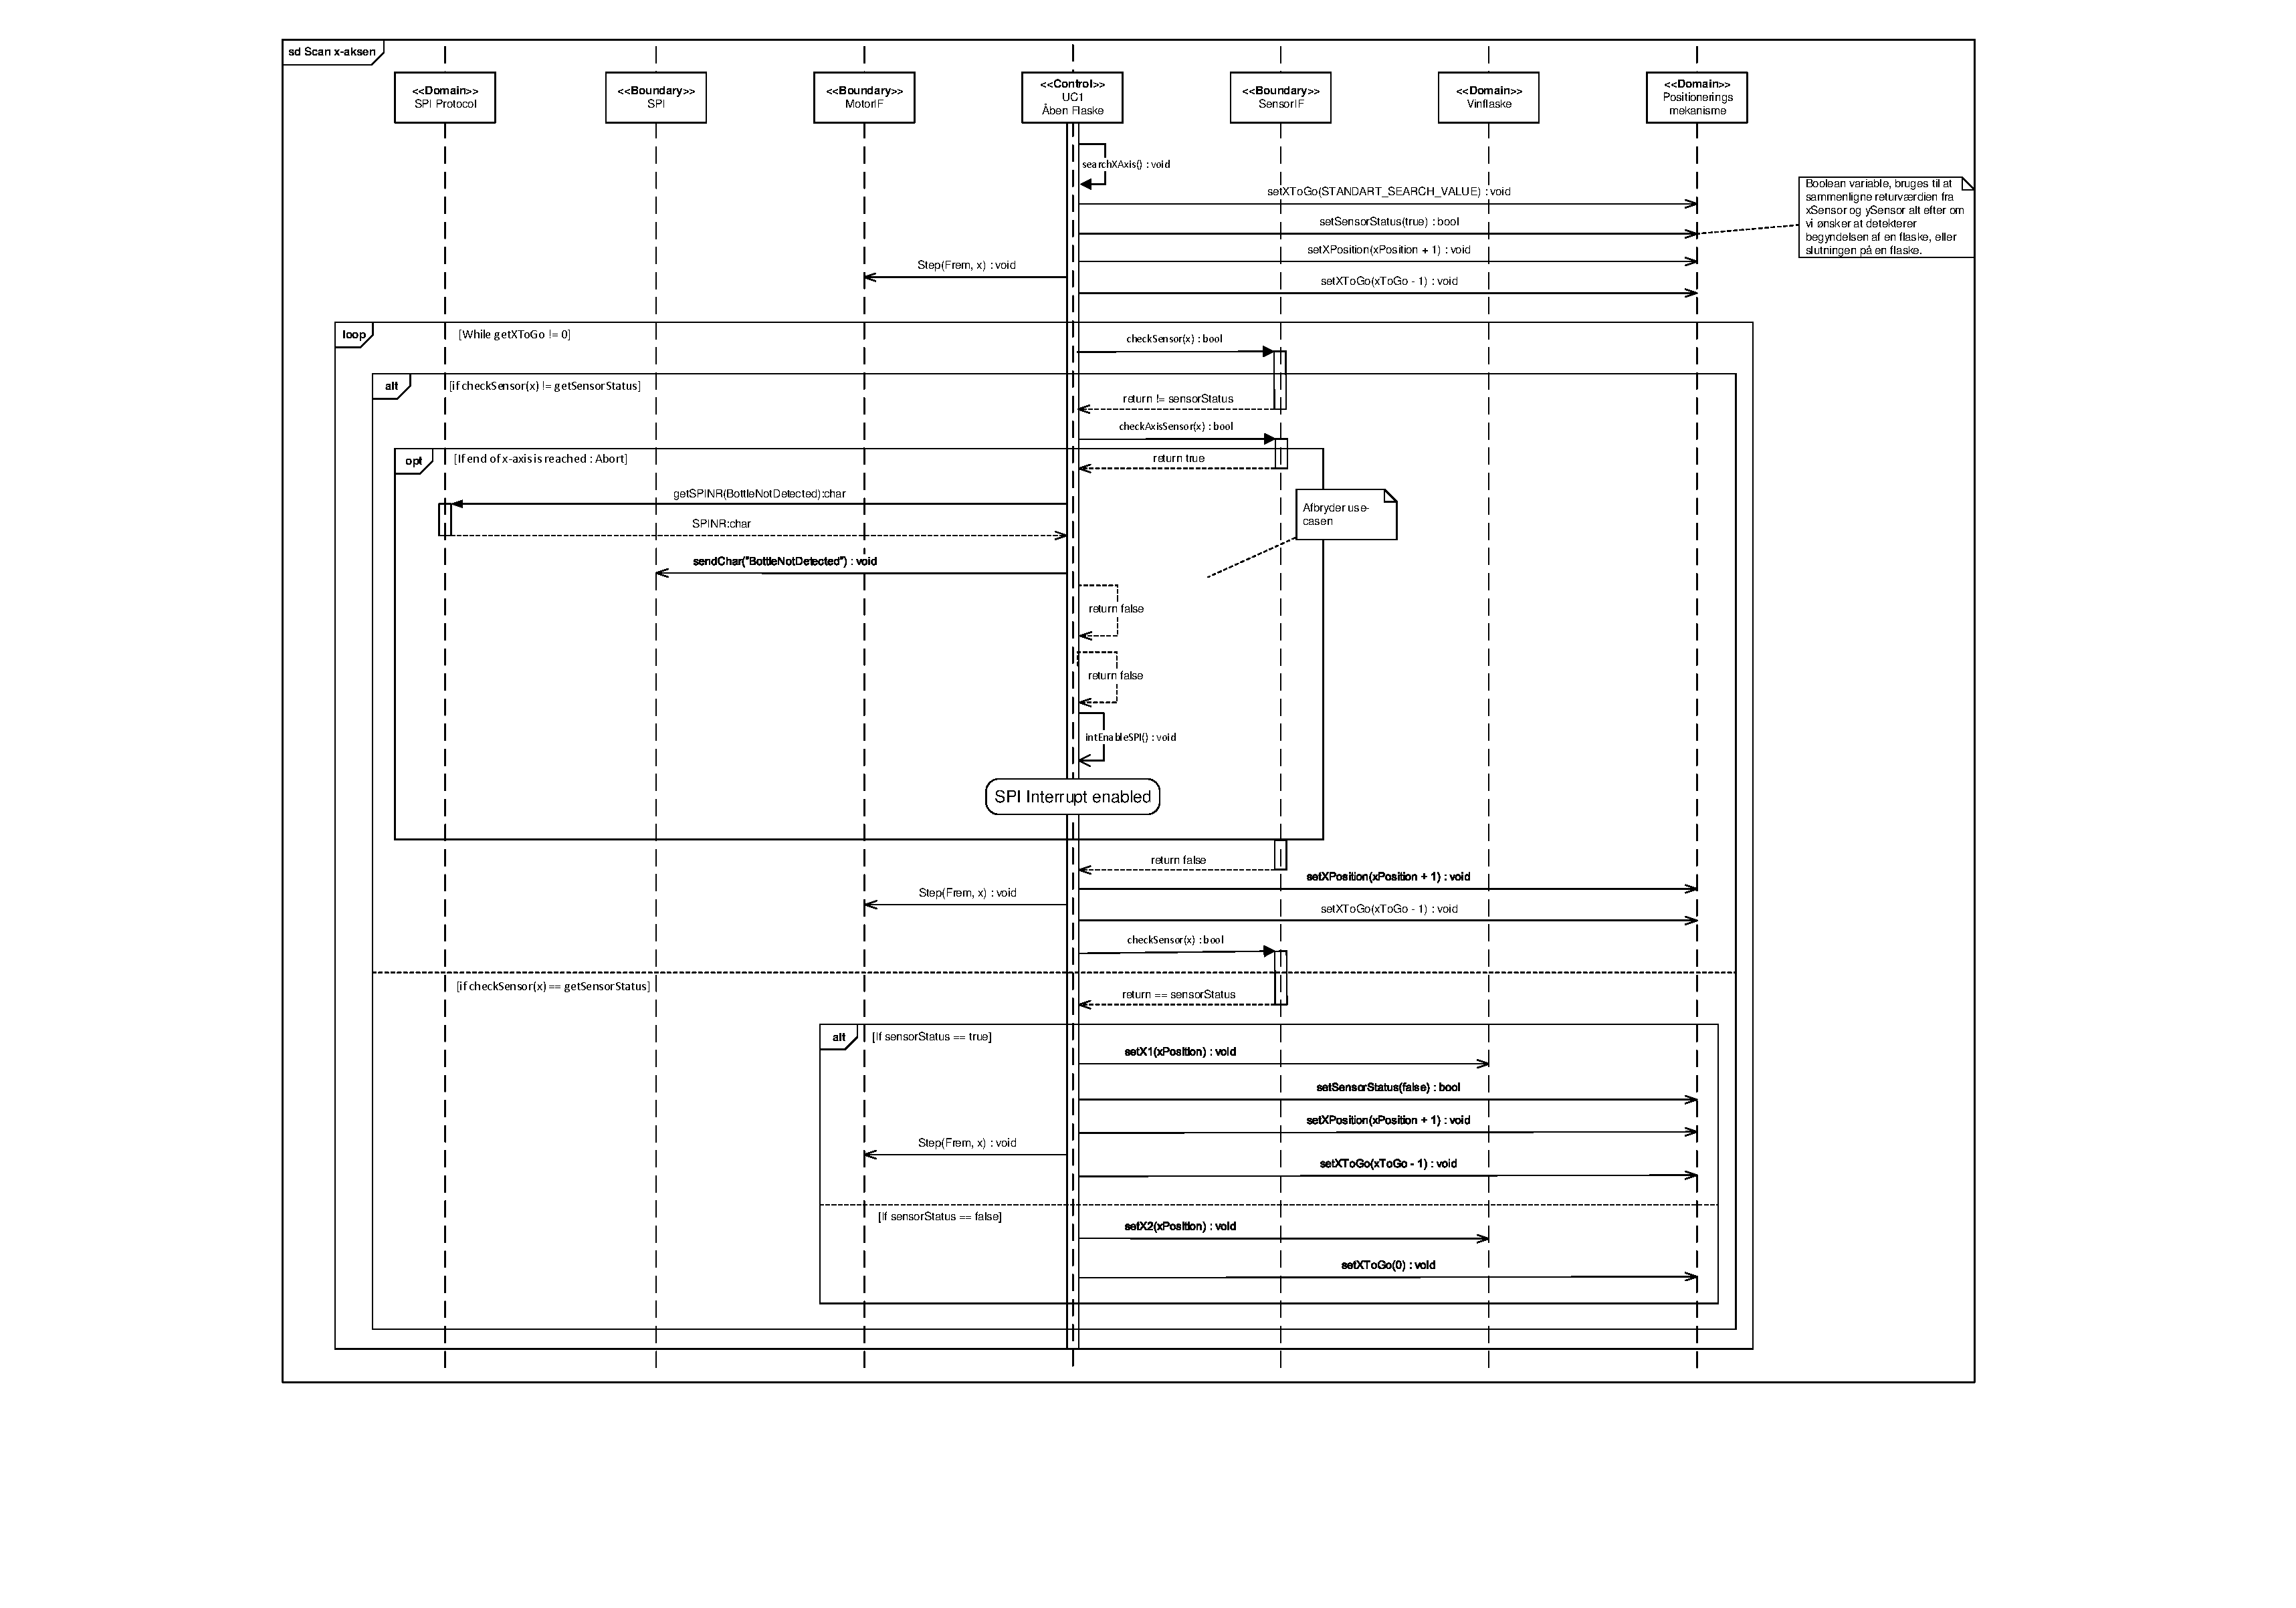
\includegraphics[scale=0.29,trim=200 150 0 0, clip]{APPSoC/SD-Scan-x-aksen}
\end{figure}

\begin{figure}[H]
	\caption{Sekvensdiagram for funktionen Scan y-aksen}
	\label{SD:PSoC:ScanY}
	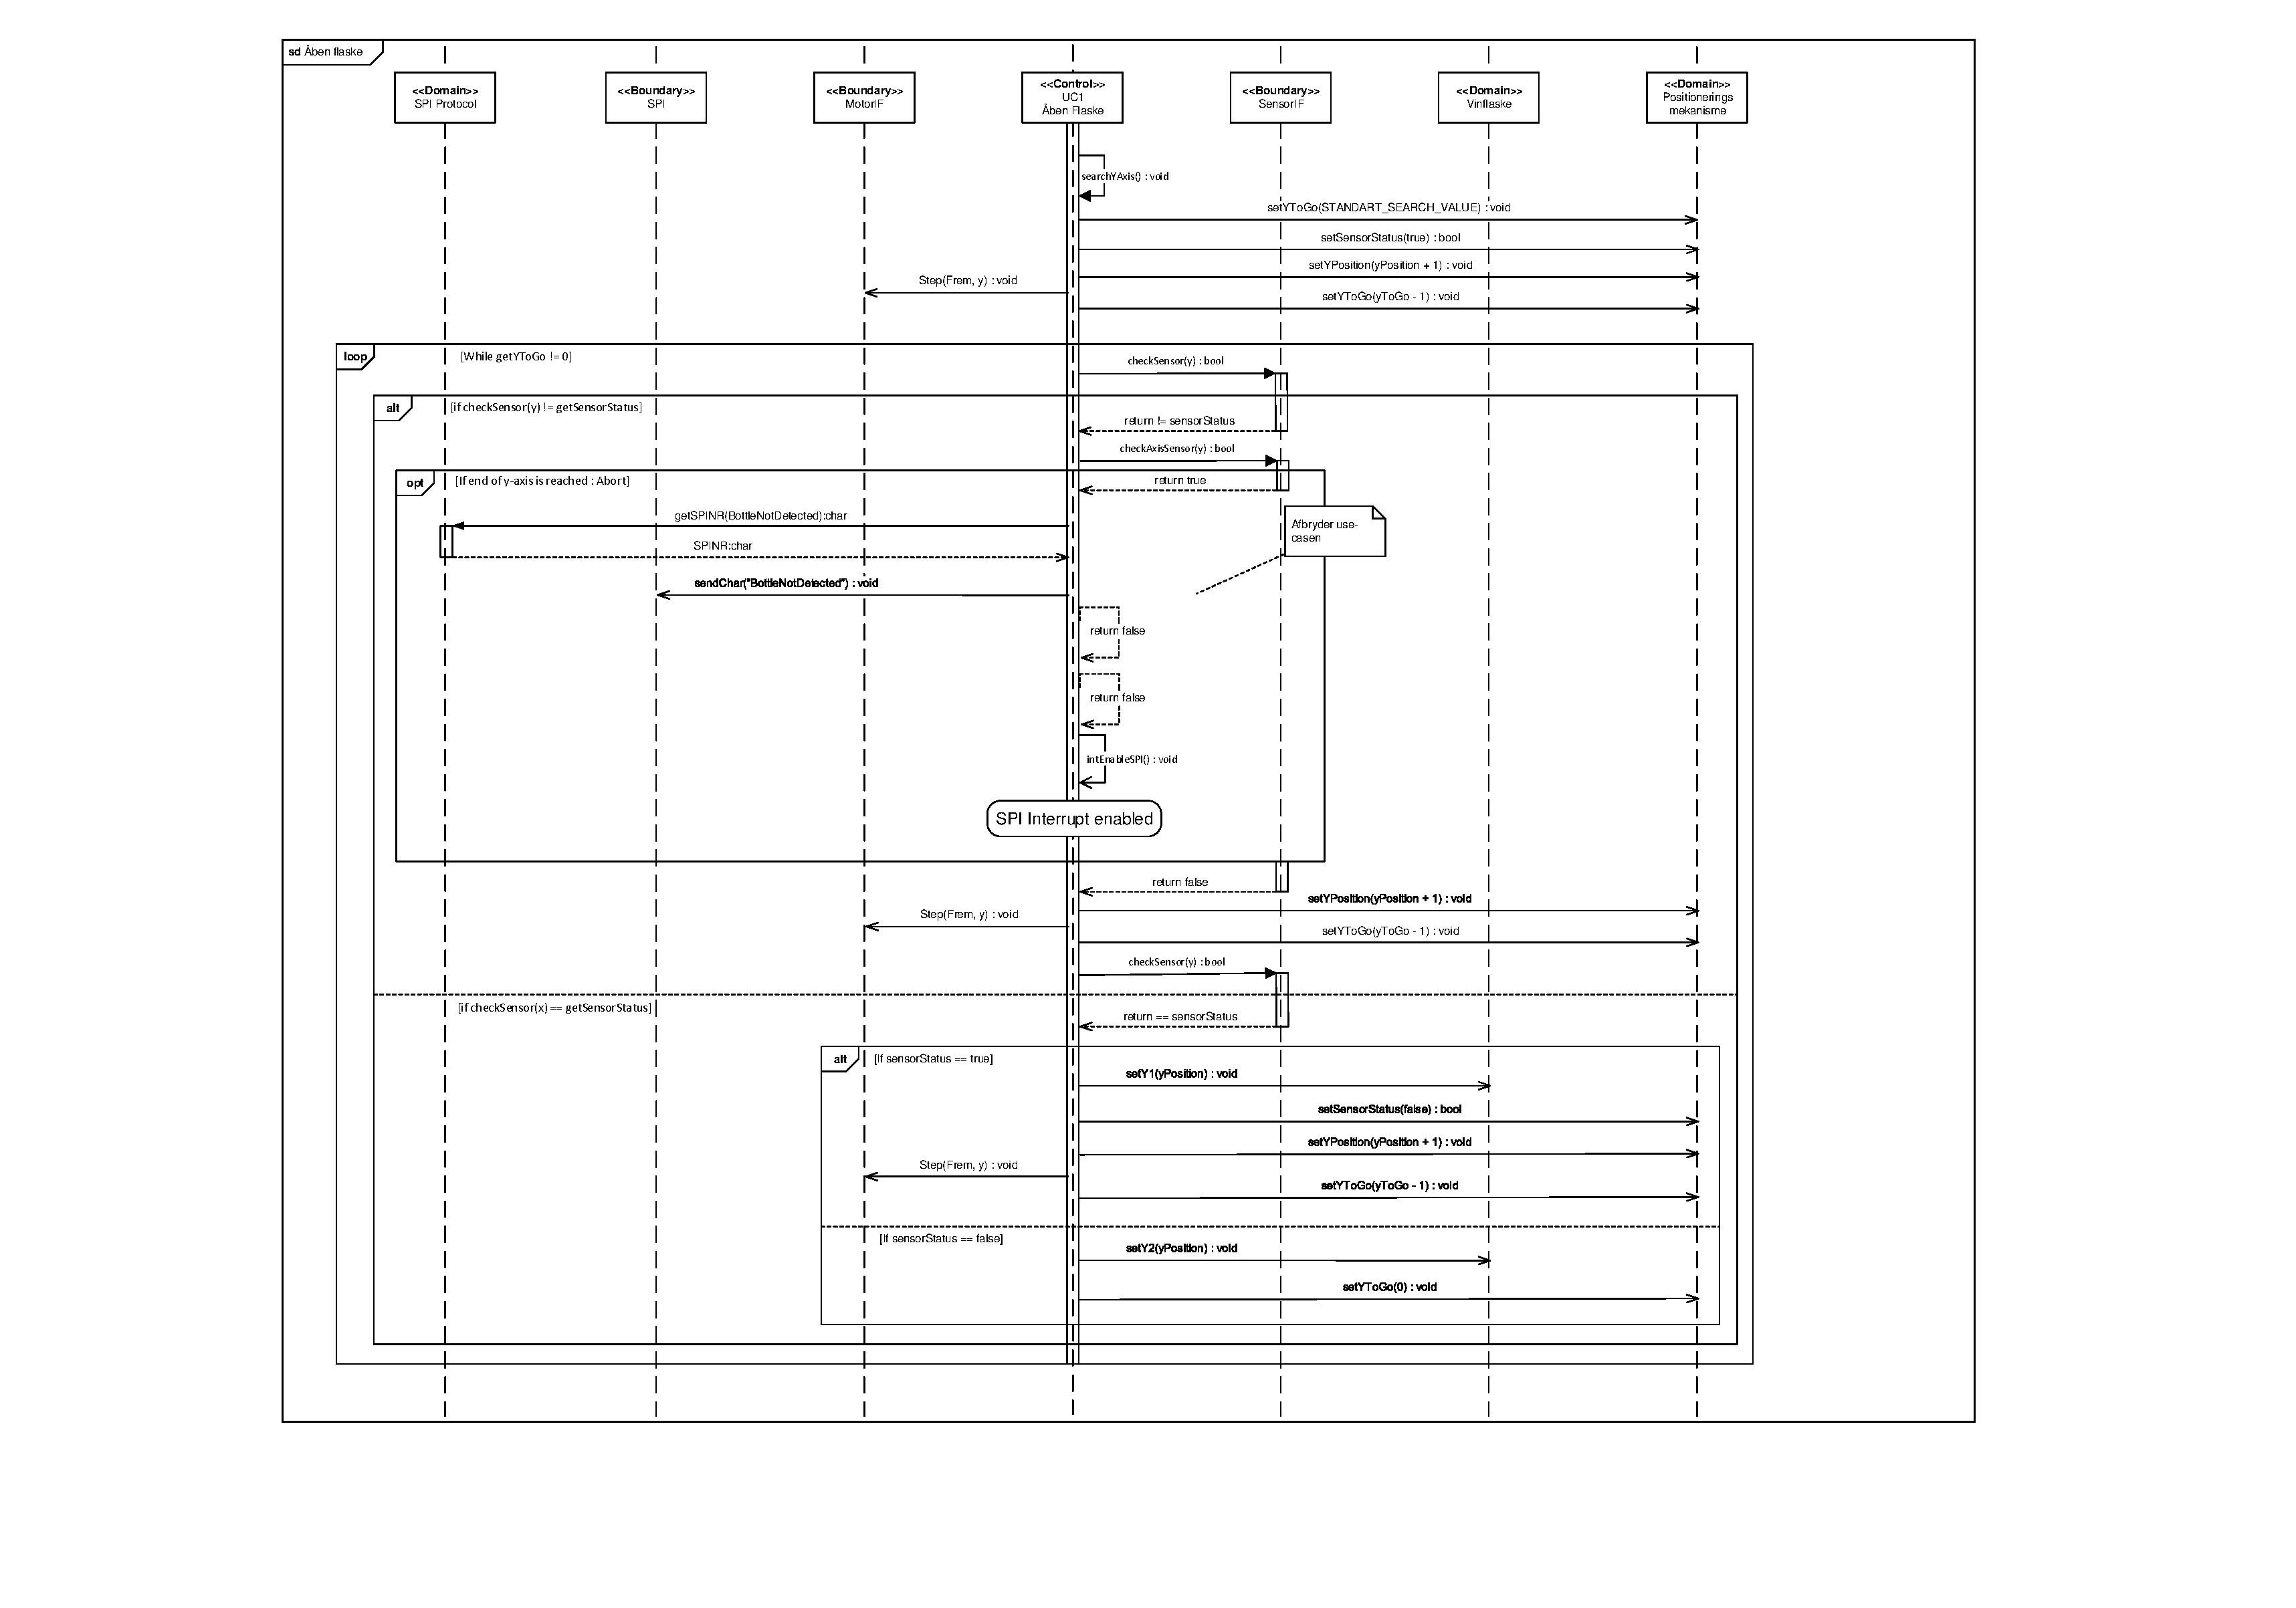
\includegraphics[scale=0.29,trim=200 100 0 0,clip]{APPSoC/SD-Scan-y-aksen}
\end{figure}

\begin{figure}[H]
	\caption{Sekvensdiagram for funktionen Scan z-aksen}
	\label{SD:PSoC:ScanZ}
	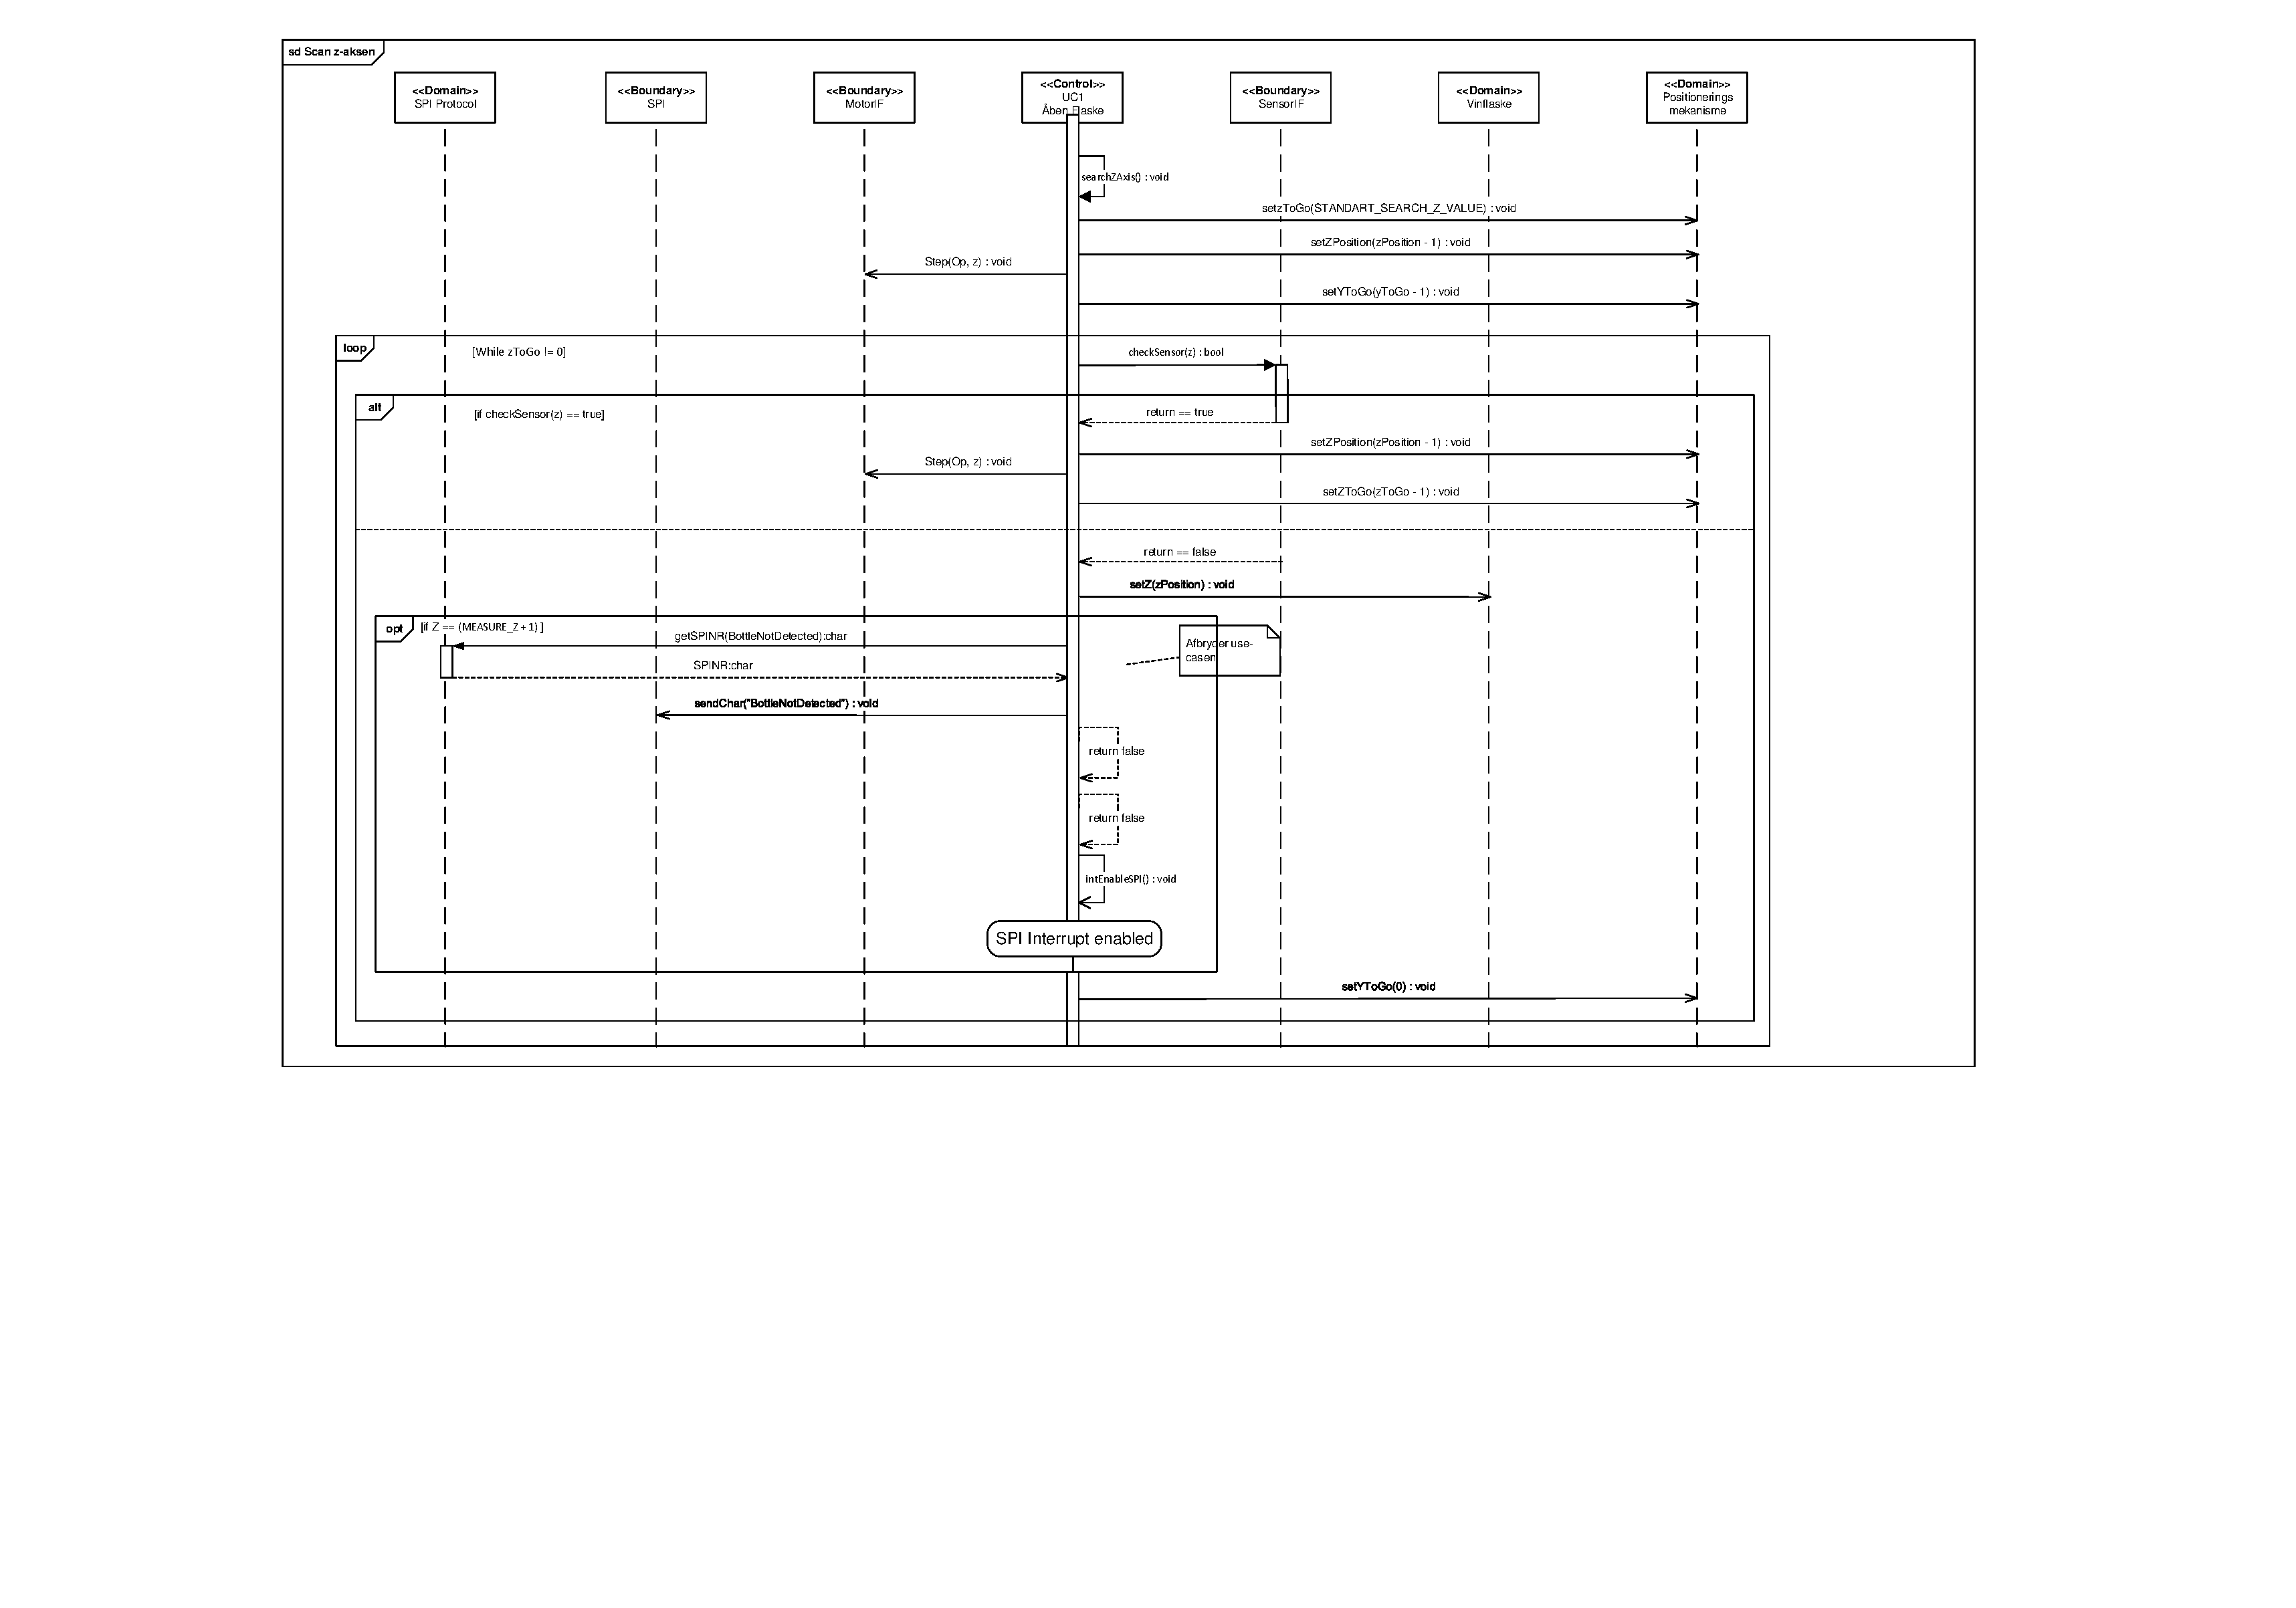
\includegraphics[scale=0.29,trim=200 100 0 0, clip]{APPSoC/SD-Scan-z-aksen}
\end{figure}